\subsection{Negative Integers:}

The fifth test will consist in evaluate the running time of the algorithms analyzing an array of disordered random negative integers of size $2^{5}$. \hfill \break

\begin{figure}[H]
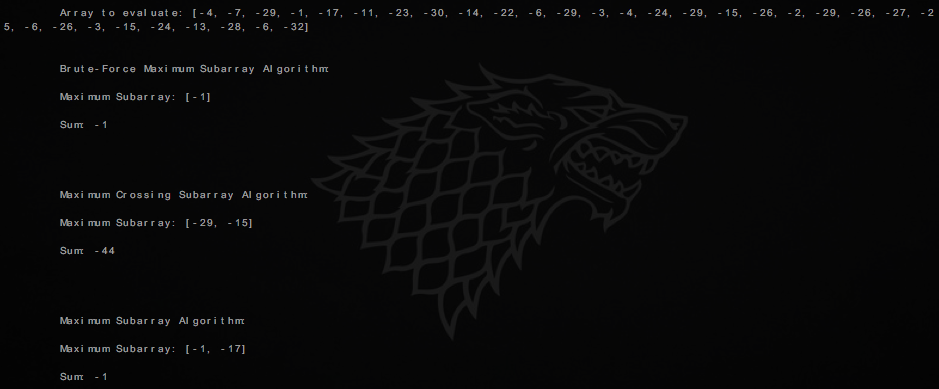
\includegraphics[width = 17cm, height = 10cm]{co5.png}
\centering \linebreak \linebreak Figure 4.3.0: Console output of the program.
\end{figure} \hfill 

\begin{figure}[H]
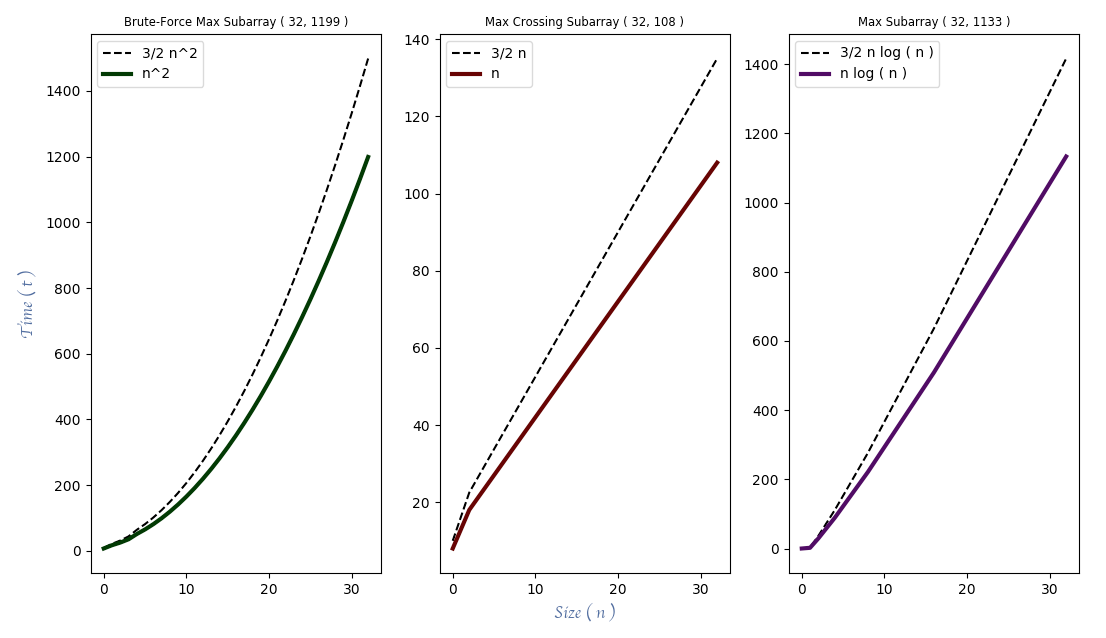
\includegraphics[width = 17cm, height = 10cm]{t5.png}
\centering \linebreak \linebreak Figure 4.3.1: Algorithms running time for an array of size $2^{5}$.
\end{figure} \hfill 

The following table shows the points of the plots where the first column it's the {\itshape Size} of the array, the second, third and fourth columns describes the computational time of {\itshape Brute-Force}, {\itshape Crossing} and {\itshape Recurrence} Maximum Subarray Algorithms respectively. \hfill \break

\begin{center} 
\begin{tabular}[.5cm]{ c c c c } 
\toprule 
\hspace{10pt} Size ( n ) \hspace{10pt} & \hspace{10pt} Brute-Force Time ( t ) \hspace{10pt} & \hspace{10pt} Crossing Time ( t ) \hspace{10pt} & \hspace{10pt} Recurrence Time ( t ) \\ 
\midrule 
0 & 7 & 8 & 0 \\ 
\cmidrule {1-4} 
1 & 17 & 13 & 2 \\ 
\cmidrule {1-4} 
2 & 25 & 18 & 29 \\ 
\cmidrule {1-4} 
3 & 35 & 21 & 59 \\ 
\cmidrule {1-4} 
4 & 51 & 24 & 89 \\ 
\cmidrule {1-4} 
5 & 65 & 27 & 122 \\ 
\cmidrule {1-4} 
6 & 81 & 30 & 155 \\ 
\cmidrule {1-4} 
7 & 99 & 33 & 188 \\ 
\cmidrule {1-4} 
8 & 119 & 36 & 221 \\ 
\cmidrule {1-4} 
9 & 141 & 39 & 257 \\ 
\cmidrule {1-4} 
10 & 165 & 42 & 293 \\ 
\cmidrule {1-4} 
11 & 191 & 45 & 329 \\ 
\cmidrule {1-4} 
12 & 219 & 48 & 365 \\ 
\cmidrule {1-4} 
13 & 249 & 51 & 401 \\ 
\cmidrule {1-4} 
14 & 281 & 54 & 437 \\ 
\cmidrule {1-4} 
15 & 315 & 57 & 473 \\ 
\cmidrule {1-4} 
16 & 351 & 60 & 509 \\ 
\cmidrule {1-4} 
17 & 389 & 63 & 548 \\ 
\cmidrule {1-4} 
18 & 429 & 66 & 587 \\ 
\cmidrule {1-4} 
19 & 471 & 69 & 626 \\ 
\cmidrule {1-4} 
20 & 515 & 72 & 665 \\ 
\cmidrule {1-4} 
21 & 561 & 75 & 704 \\ 
\cmidrule {1-4} 
22 & 609 & 78 & 743 \\ 
\cmidrule {1-4} 
23 & 659 & 81 & 782 \\ 
\cmidrule {1-4} 
24 & 711 & 84 & 821 \\ 
\cmidrule {1-4} 
25 & 765 & 87 & 860 \\ 
\cmidrule {1-4} 
26 & 821 & 90 & 899 \\ 
\cmidrule {1-4} 
27 & 879 & 93 & 938 \\ 
\cmidrule {1-4} 
28 & 939 & 96 & 977 \\ 
\cmidrule {1-4} 
29 & 1001 & 99 & 1016 \\ 
\cmidrule {1-4} 
30 & 1065 & 102 & 1055 \\ 
\cmidrule {1-4} 
31 & 1131 & 105 & 1094 \\ 
\cmidrule {1-4} 
32 & 1199 & 108 & 1133 \\ 
\bottomrule 
\linebreak 
\end{tabular} 
\linebreak \linebreak Table 4: Plot points of Figure 4.3.1.
\end{center} \hfill 

\pagebreak

The sixth test will consist in evaluate the running time of the algorithms analyzing an array of disordered random negative integers of size $2^{4}$. \hfill \break

\begin{figure}[H]
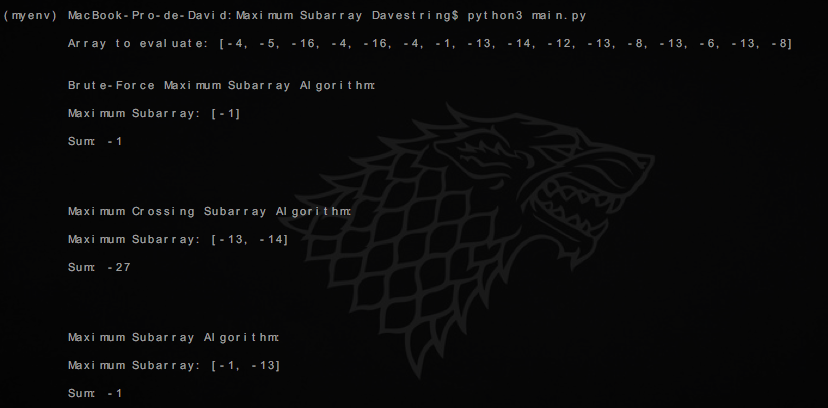
\includegraphics[width = 17cm, height = 10cm]{co6.png}
\centering \linebreak \linebreak Figure 4.3.2: Console output of the program.
\end{figure} \hfill 

\begin{figure}[H]
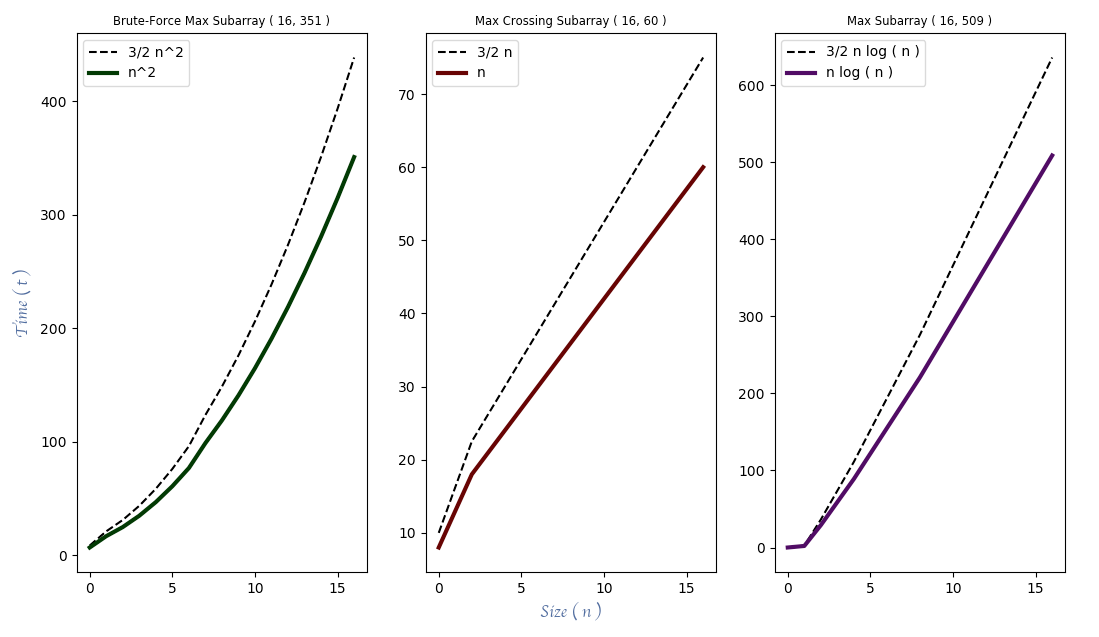
\includegraphics[width = 17cm, height = 10cm]{t6.png}
\centering \linebreak \linebreak Figure 4.3.3: Algorithms running time for an array of size $2^{4}$.
\end{figure} \hfill 

The following table shows the points of the plots where the first column it's the {\itshape Size} of the array, the second, third and fourth columns describes the computational time of {\itshape Brute-Force}, {\itshape Crossing} and {\itshape Recurrence} Maximum Subarray Algorithms respectively. \hfill \break

\begin{center} 
\begin{tabular}[.5cm]{ c c c c } 
\toprule 
\hspace{10pt} Size ( n ) \hspace{10pt} & \hspace{10pt} Brute-Force Time ( t ) \hspace{10pt} & \hspace{10pt} Crossing Time ( t ) \hspace{10pt} & \hspace{10pt} Recurrence Time ( t ) \\ 
\midrule 
0 & 7 & 8 & 0 \\ 
\cmidrule {1-4} 
1 & 17 & 13 & 2 \\ 
\cmidrule {1-4} 
2 & 25 & 18 & 29 \\ 
\cmidrule {1-4} 
3 & 35 & 21 & 59 \\ 
\cmidrule {1-4} 
4 & 47 & 24 & 89 \\ 
\cmidrule {1-4} 
5 & 61 & 27 & 122 \\ 
\cmidrule {1-4} 
6 & 77 & 30 & 155 \\ 
\cmidrule {1-4} 
7 & 99 & 33 & 188 \\ 
\cmidrule {1-4} 
8 & 119 & 36 & 221 \\ 
\cmidrule {1-4} 
9 & 141 & 39 & 257 \\ 
\cmidrule {1-4} 
10 & 165 & 42 & 293 \\ 
\cmidrule {1-4} 
11 & 191 & 45 & 329 \\ 
\cmidrule {1-4} 
12 & 219 & 48 & 365 \\ 
\cmidrule {1-4} 
13 & 249 & 51 & 401 \\ 
\cmidrule {1-4} 
14 & 281 & 54 & 437 \\ 
\cmidrule {1-4} 
15 & 315 & 57 & 473 \\ 
\cmidrule {1-4} 
16 & 351 & 60 & 509 \\ 
\bottomrule 
\linebreak 
\end{tabular}  
\linebreak \linebreak Table 5: Plot points of Figure 4.3.3.
\end{center} \hfill 

\pagebreak
